\chapter{Methodology}
\section{Introduction}
Cyberspace is the digital creativity environment in which we live and
which is controlled by cybersecurity.  Perhaps the basic vision of
cybersecurity is to reach a \emph{virtuous} digital world.  In order to
reach such a strategic goal, the mission of cybersecurity must be how
to insert human ethics and values into software values.  This matter
in itself is not easy at all because it requires an ethical philosophy
related to cybersecurity.  This philosophy proposes that cyberspace
be an \emph{ideal} alternative to the real world as much as possible.
What we mean by \emph{idealism} here is that the presence of each member
in this space is effective and not harmful to others.  To achieve this
requires answering two important questions.

\begin{enumerate}
\item What is the current presence of members in cyberspace? And,
\item how can this presence be digitally enhanced to be ideal?
\end{enumerate}

Through this chapter, we tried to provide a convincing answer to both
questions by developing a  logical framework for cybersecurity. 
%that proposes stakeholder policies and a social contract of cyberspace.



\section{Logical analysis}
%-------from hand book-ch1-1.3 Methodology begin
Although the science and art of computing, and of communication, form the foundation on which cybersecurity rests, we cannot use these disciplines to explain or unlock the mysteries of cybersecurity. Also, much as number theory has a special place in the world of cybersecurity, it does not provide skills or ideas of the sort that are relevant regularly to cybersecurity professionals. But there is an area of mathematics that is relevant to almost every attack, not just upon encrypted communication, but all cyber-attacks. 

This area is {\em logic}. The concept of {\em logic} is relevant to everyone, and all fields of human endeavour. The importance of logic is imposed, by reality, by anyone who ignores it. Conseqently, everyone has a basic understanding of logic. What varies, from one to another, is not so much understanding of logic, as awareness of when it is in use. Not everyone is self-conciously {\em aware} when they are using logic.

This extra step of {\em self-aware application} of logic is not always necessary but helps in cases of critical importance, where getting details wrong can sometimes cause serious harm. In cybersecurity, as in pure mathematics, the consequences of minor logical mistakes can sometimes be disastrous. 

This is why, in this dessertation, {\em mathematical} logic is regarded as the key scientific method which we employ to analyse cybersecurity problems, and in the design of cybersecurity solutions.
\if
This is not meant to suggest that mathematical logic should be used on a regular basis by cybersecurity professionals. Many cybersecurity professionals will never use it, and currently, many may not even have heard ot it. However, {\em logic} is used by all cybersecurity professionals on a regular basis. In the course of understanding how this takes place, and how it is done consistently and correctly, with as little chance of error as possible, we need to develop the sort of self-awareness, of what we are doing, that is best characerised, and explained, in the particular form of logic known as mathematical logic.\index{logic!mathematical}
%-------from hand book-ch1-1.3 Methodology end
\fi
[One of the methods used in this work is to apply logic to cybersecurity objectives. 

In particular, logic can be used to show {\em how} cybersecurity objectives can
be met. Logic is the appropriate tool, for example, if the objective sought can
be shown to follow, logically, from certain other rules.

In some cases it may also be possible, and useful, to show that certain objectives can {\em only}
be met in certain ways.]

In this section, we developed concepts and tools which assist cybersecurity professionals to define the mandatory objectives of their systems, the rules which enforce these objectivities, and the reasoning behind the choice of these rules. The concepts and tools we proposed and illustrated in this section will be shown, in Chapter 5, to be sufficient to record and analyse these rules, both the objectives and the rules which are enforced, and to ensure that there are no logical flaws in the system which has been designed. Note that we assume our cybersecurity objectives include the control of all important risks. 

%Hand book-----ch2 begin
\subsection{Logic}\label{logicsec}\index{logic}

Assuming we have discovered and expressed all the conditions for the mandatory objectives for our organization, how do we now ensure that they hold? There are some conditions that we can impose directly. For example, door locks can be installed which require key-cards, which are issued to all employees. This enforces a condition: 
\begin{quote}\em
People entering a building must posess a key card.
\end{quote}
(For the moment, let us ignore the possibility that two people enter at once, after presentation of a single key-card.)

There are many conditions that can be directly enforced. However, most of the conditions that we seek to ensure are not directly enforceable but instead will depend on a number of other conditions in a complicated web of logical connections.

Everyone uses logic on a daily basis. Reality imposes logic upon us; consistently, and hence no one deviates {\em too} far from being logical. Despite this, there are areas of our professional lives where the need for logic is somewhat greater, and at the same time there are pressures, and biases, that tend to create a counter-pressure that enables sloppy or lazy thinking, and hence inhibits logic from fully functioning as it needs to in our decision making. For example, it may be company policy to publicly reveal all breaches of client privacy as soon as they occur, but such revelations will usually also reveal one or more faults or breaches of correct practices, and there may be many individuals who are personally disadvantaged by publicly revealing these faults or breaches.

Also, there are a number of logical fallacies that regularly occur in the way we think which we can't afford to allow to compromise our decision-making in the area of security.

Security is an area where there is a need for clear thinking, free of influence from other goals, be they personal, financial, or something else. This is a practical explanation of why, in this dissertation, logic is adopted as the key discipline on which we can base our investigation, and development, of a methodology for cyber-security.

\subsection{Propositional Logic}\index{propositional logic}

In Propositional logic, there are certain basic propositions about which we argue, or develop deductions, 
which are {\em atomic}, i.e. we do not attempt to break these basic propositions down further. For this reason,
these propositions have {\em names}, but no internal details. Some propositions can be analysed into {\em combinations}
of other propositions, formed from component propositions and operators which apply to these. The most important
logical operators are `and' ($\wedge$), `or' ($\vee$), `not' ($\neg$), and `implies' ($\supset$).

If $p_1$ and $p_2$ are two propositions, $p_1\wedge p_2$ denotes the proposition $p_1$ {\em and} $p_2$,
$p_1 \vee p_2$ denotes the proposition $p_1$ {\em or} $p_2$, 
$\neg p_1$ denotes the proposition not $p_1$, and $p_1 \supset p_2$ denotes
the proposition $p_1$ {\em implies} $p_2$.

Propositional variables, like $p_1$ and $p_2$, are assumed to take one of the two values true, or false.
In some instances, the propositional variables may have the same {\em meaning}, in an informal sense,
in two situations, and yet take different values in each case. For example, $p_1$ might denote ``John has
had breakfast''.  This proposition might be false at 6.00am and true at 9.00am. As far as logic is concerned,
these are two different propositions, but nevertheless, the same logical framework can apply in two
different contexts, and for this reason, and others, it is useful to use variables to denote truth values in this way.


\begin{sbexample}{An example of a formal system}\label{certificatesex}%
Suppose we have the following propositions:
\begin{eqnarray}\nonumber
\textup{$p_1$}: &&\parbox{10cm}{Document $d$ of Joan is correctly signed by Joan.}\\\nonumber
\textup{$p_2$}:&& \parbox{10cm}{The certificate of Joan is correctly signed by CertiSign.}\\\nonumber
\textup{$p_3$}:&& \parbox{10cm}{CertiSign has a certificate.}\\\nonumber
\textup{$p_4$}:&& \parbox{10cm}{The certificate of CertiSign has a valid signature.}\\\nonumber
\textup{$p_5$}:&& \parbox{10cm}{Joan is a signatory of document d.}
\end{eqnarray}

Informally, from $p_1$, $p_2$, $p_3$ and $p_4$, we can conclude $p_5$. However, we would like to 
elaborate a more formal proof that statement $p_5$ follows from $p_1$, \dots, $p_4$. To do this
we need to make some assumptions, which in the language of formal logic, are known as {\em axioms}.
It may seem that by adopting these axioms we have somehow bypassed the real work of proving $p_5$.
However, from the point of view of formal logic, it is precisely the task of {\em finding the
right axioms}, that is at the heart of correctly understanding and analysing the logical underpinnings of
any subject.

{\bf Proposed Axioms for Certificates}
\begin{itemize}
	\item[A1] A certificate is {\em valid} if it's signature is a valid hash of 
		the certificate document when checked by the public certificate of
		the signing authority and the signing authority is valid.
	\item[A2] Entity $P$ is a signatory of document $d$ if the public certificate of $P$
		is valid and the signature attached to it is a valid hash of $d$ when checked by that certificate.
	\item[A3] A signing authority with a valid public certificate is valid.
	\item[A4] Verisign is a valid signing authority.
\end{itemize}

To prove $p_4$ we are going to need some additional {\em intermediate} propositions, namely:
\begin{eqnarray}
		p_6:&&\hbox{The public certificate of Certisign is a valid.}\nonumber\label{v1}\\
		p_7:&&\hbox{Certisign is a valid signing authority.}\nonumber\label{v1}\\
		p_8:&&\hbox{Joan's certificate is valid.}\nonumber\label{v1}
\end{eqnarray}

{\bf Proof}
\begin{enumerate}[1.]
\item $p_6$ follows from A1, A4 and $p_3$. 

\item $p_7$ follows from $p_6$ and A3. 

\item $p_8$ follows from $p_7$ and A1. 

\item Lastly, $p_5$ then follows from A2, $p_8$, and $p_1$.
\end{enumerate}

{\bf Comments}

Each of the {\em deductions} in this proof is a valid interpretation of the propositions. For example,
in Line 1 of the proof,
A1 gives conditions under which a certificate is valid, the other two propositions invoked ensure
that these conditions are valid, and hence the conclusion of A1 is valid, and this is $p_5$. However,
we have not yet formalised the concept of {\em deduction}. In fact, this example requires the additional
concepts which will be introduced in the next subsection for the full concept of deduction
that needs to be explained here.

In particular, we also need the concept of a {\em domain} of objects, to which our propositions
apply. In natural languages, the sentences are not atomic constructs with nothing more than a name, but
are composed of {\em words}, some of which refer to {\em objects}. Some of these objects play the role of
{\em actors}, syntactically appearing as a {\em subject}, and others play a more passive role, and these
play the role of {\em object}. In most languages, every sentence also contains a {\em verb}. To
go some way toward this level of detail, in the {\em predicate calculus}, we have a domain
of objects, and a collection of predicates, which apply to these objects. After these concepts
have been introduced, in Section \ref{predicatesec}, we shall revisit this example 
-- in Example \ref{predicatesex} -- and make use of a domain
and predicates to define the the axioms, assumptions, and statements to be proved, more precisely.

\end{sbexample}

The connectives ($\vee$, $\wedge$, $\supset$, and $\neg$) of Propositional calculus can be defined
by {\em truth tables}, as shown in Tables \ref{veetable}--\ref{nottable}.
\begin{table}
\begin{minipage}{0.5\linewidth}
\begin{center}
\caption{Truth table for $\vee$}\label{veetable}~\\[5mm]
\begin{tabular}{|c|c|c|}
\hline
$ a$&$ b$&\bf $a\vee b$\\
\hline
T & T& T\\
F & T& T\\
T & F& T\\
F & F& F\\
\hline
\end{tabular}
\end{center}
\end{minipage}
\begin{minipage}{0.5\linewidth}
\begin{center}
\caption{Truth table for $\wedge$}\label{wedgetable}~\\[5mm]
\begin{tabular}{|c|c|c|}
\hline
$ a$&$ b$&\bf $a\wedge b$\\
\hline
T & T& T\\
F & T& F\\
T & F& F\\
F & F& F\\
\hline
\end{tabular}
\end{center}
\end{minipage}
\end{table}

\begin{table}
\begin{minipage}{0.5\linewidth}
\caption{Truth table for $\supset$}\label{imptable}~\\[5mm]
\begin{center}
\begin{tabular}{|c|c|c|}
\hline
$ a$&$ b$&\bf $a\supset b$\\
\hline
T & T& T\\
F & T& T\\
T & F& F\\
F & F& T\\
\hline
\end{tabular}
\end{center}
\end{minipage}
\begin{minipage}{0.5\linewidth}
\caption{Truth table for $\neg$}\label{nottable}~\\[5mm]
\begin{center}
\begin{tabular}{|c|c|}
\hline
$ a$&\bf $\neg a$\\
\hline
T & F\\
F & T\\
\hline
\end{tabular}
\end{center}
\end{minipage}
\end{table}

Using these tables, we can make truth tables for any expression involving a finite number of propositional
variables. Such a formula which alway takes the value {\em true}, is called a {\em tautology}. For example,
$p\supset p$ or $p \vee \neg p$, $\neg (p\wedge\neg p)$.

Another way to determine all the true statements from the Propositional Calculus is to start with a finite
set of {\em axioms}\index{axiom} (all of which are tautologies), and generate all other true statements from these by
means of one or more rules. There is a specific rule which has traditionally been used, known as {\em modus ponens}\index{modus ponens},
which is can be written:
\begin{equation}\label{modusponens}
A, A \supset B \vdash B.
\end{equation}
The symbol $\vdash$ can be read: ``is sufficient to deduce''. In words (\ref{modusponens})
says: ``We can infer $B$ from $A$ and $A\supset B$.

A sufficient set of axioms to be able to generate all the tautologies of the Propositional calculus, by
just using modus ponens, is as follows \cite{Kleene52}:
\begin{eqnarray}\label{A->B->A}
&&A \supset (B\supset A) \\ \label{Ax1b}
&&(A\supset B) \supset ((A \supset (B\supset C))\supset(A\supset C))  \\
\label{^inf}
&&A \supset (B \supset A \wedge B) \\
		\label{a&b->a}
&&A\wedge B \supset A \\
		\label{a&b->b}
&&A\wedge B \supset B \\
&&A\supset A \vee B \\
&&B\supset A \vee B \\
&&(A \supset C) \supset ((B\supset C) \supset (A\vee B \supset C)) \\
\label{2ndlastaxiom}
&& (A \supset B) \supset ((A\supset \neg B) \supset \neg A) \\\label{negneg}
&& \neg\neg A \supset A.
\end{eqnarray}

It is not obvious that these axioms, together with the rule modus ponens, is sufficient
to deduce all the true statements of the propositional calculus. This is shown, however,
in \cite[Theorem 10]{Kleene52}.

Each of (\ref{A->B->A})--(\ref{negneg}) is a {\em schema}
for axioms, not just one specific axiom. For example, in the case of Axiom (\ref{A->B->A}),
we can substitute any syntactically valid formula for A, and any {\em other} syntactically valid formuls
for B. The formulae substituted for A must all be the same. For example,
$$
\neg\neg C \supset (\neg D \supset \neg\neg C)
$$
is an {\em instance} of axiom (\ref{A->B->A}).

\subsection{Some Important Reasoning Methods}\label{reasoningmethods}

Although proofs can be constructed by sequences of statements, annotated by explanations of the reasoning,
in practice we use some higher level arguments which make the reasoning easier to follow. Two
of these higher level methods are now introduced: the {\em deduction theorem} \cite[\S 21--22]{Kleene52}
and {\em proof by contradiction}. The first is the deduction theorem:

\begin{theorem}\index{deduction}
If $\Gamma$, $A \vdash B$ then $\Gamma \vdash A \supset B$.
\end{theorem}

\begin{proof}
See \cite[\S 21--22]{Kleene52}.
\end{proof}

The following is a version of proof by contradiction, or, in the latin, {\em reductio ad absurdum}\index{contradiction}.
\begin{theorem}\label{reductioadabsurdum}
If $\Gamma$, $\neg A \vdash B$ and also $\Gamma$, $\neg A \vdash \neg B$ then $\Gamma \vdash A $.
\end{theorem}

\begin{proof}
See \cite[Theorem 2]{Kleene52}.
\end{proof}

There are several more convenient and natural rules of deduction presented 
in \cite[Theorem 2]{Kleene52}. These are presented in Table \ref{Kleenerules}.
Using these rules makes it a lot easier to explain a logical argument. Most of these rules
are regularly used in rational discussion in the normal course of life. Some rules are a little
more specialized, but even in these cases the correctness of the deduction is obvious
to anyone with higher education. The real challenge in using these rules is being
sufficiently self-aware to recognise that they are being used.

In this table, $\Gamma$ denotes a {\em set} of statements. Each rule forms a pair with
another rule, with one of them termed {\em introduction} and the other {\em elimination}.
For example, {\em Conjunction introduction} allows us to deduce $A\wedge B$ from $A$ together with $B$,
while {\em Conjunction elimination} allows us to deduce $A$ from $A\wedge B$, and also $B$ from $A\wedge B$.
In the case of the rule {\em Generalization}, it is the quantifier ($\forall$) which is being eliminated
and a more natural name for the elimination version of this rule is {\em Specialization}.
\begin{table}
		\centering
		\caption{Expanded rules of deduction}\label{Kleenerules}
		\begin{tabular}{|p{5cm}|p{5cm}|}
				\hline
		\bf Introduction & \bf Elimination\\
				\hline
		(Implication) If $\Gamma, A \vdash B$, then $\Gamma \vdash A\supset B$. &
		$A, A\supset B \vdash B$ (Modus ponens).\\
				\hline
		(Conjunction) $A, B \vdash A \wedge B$. & $A\wedge B \vdash A$, $A\wedge B \vdash B$\\
				\hline
		(Disjunction) $A \vdash A \vee B $, $B \vdash A \vee B $ . & If $\Gamma$, $A\vdash C $ and $\Gamma$, $B \vdash C$,
				then $\Gamma, A\vee B \vdash C$ (Proof by cases).\\
				\hline
		(Negation) If $\Gamma$, $A \vdash B$ and $\Gamma$, $A \vdash \neg B $ 
				then $\Gamma \vdash \neg A$ (Proof by contradiction) & $\neg\neg A \vdash A$.\\
				\hline
		(Generalization) $A(x) \vdash \forall xA(x)$ & (Specialization) $\forall x A(x) \vdash A(t)$.\\
				\hline
		(Existence) $A(t) \vdash \exists x A(x)$ & If $\Gamma(x)$, $A(x) \vdash C$, then
				$\Gamma(x)$, $\exists x A(x) \vdash C$.\\
				\hline
\end{tabular}
\end{table}
%

An important consequence of Theorem \ref{reductioadabsurdum} is that if $\Gamma\vdash B$ and $\Gamma\vdash\neg B$,
any statement at all can be proved from $\Gamma$, i.e. all statements are provable. In this case we say $\Gamma$ 
is {\em inconsistent}. Consistency is a very important property of any theory. Without it, the theory is of
little use. Consistency is considered in more detail in Subsection \ref{consistencysec}.

\begin{sbexample}{Some theorems}\label{sometheorems}%
\begin{enumerate}[(i)]
\item\label{a->a} $A \supset A$;\\
{\em Proof:}
\begin{eqnarray}\label{i1}
\hspace{-4cm}&&A \supset (A \supset A)\\
\noalign{from (\ref{A->B->A})}
\label{i2}
\hspace{-4cm}&&(A\supset(A\supset A)) \supset ((A \supset ((A\supset A)\supset A))\supset(A\supset A))  \\
\noalign{from (\ref{Ax1b}), using $A\supset A$ in place of B, and A in place of C}
\label{i3}
\hspace{-4cm}&& (A \supset ((A\supset A)\supset A))\supset(A\supset A)  \\
\noalign{modus ponens with (\ref{i1}) and (\ref{i2})}
\label{i4}
\hspace{-4cm}&&A\supset ((A\supset A)\supset A) \\
\noalign{from (\ref{A->B->A})}
\hspace{-4cm}&&A \supset A\\ 
\noalign{by modus ponens, again, this time using (\ref{i4}) and (\ref{i3}).}
\nonumber\hspace{-4cm}&&
\end{eqnarray}

\item\label{converse} $(A\supset B) \supset (\neg B \supset \neg A)$;\\
{\em Proof:}
Suppose $A\supset B$ and $\neg B$. 
Using (\ref{A->B->A}), $\vdash A\supset \neg B$.
Thus, by (\ref{2ndlastaxiom}), $\vdash \neg A$. Hence, the deduction theorem, $\vdash \neg B \supset \neg A$.
Using the deduction theorem again we obtain the stated result.

\item\label{infjoin} $A, B \vdash A \wedge B$.\\
{\em Proof:}
\begin{eqnarray}\label{iii1}
\hspace{-4cm}&&A, (\ref{^inf}) \vdash B \supset (A \wedge B) \\
\noalign{modus ponens}
\hspace{-4cm}&&B, (\ref{iii1}) \vdash A \wedge B
\end{eqnarray}
by modus ponens, again.

\end{enumerate}
\end{sbexample}

\begin{exercise}{One more theorem}%
Prove
$\neg\neg\neg A \supset \neg A$.
\end{exercise}

\subsection{The Predicate Calculus}\label{predicatesec}\index{predicate calculus}

The range of systems that can be modelled with the propositional calculus is
very limited. In particular, it lacks the concept of a domain of objects about which
statements are being made. The predicate calculus \cite{Mendelson64} adds the concept of {\em predicate},
which is a symbolic statement about one or more objects, e.g. $P(a,b)$. In this example,
$P$ is the predicate, and $a$ and $b$ are objects. Although we will often find it useful
to ascribe a meaning to such predicates, for example we might say $P(a,b)$ means, intuitively,
that $a$ is a parent of $b$, there is no formal mechanism within the predicate calculus
for assigning a meaning to predicates. In effect, this is left to the much less direct
impact of the axioms which we select and then analyse, which the predicates of a system
are subject to.

The predicate calculus also adds the concept of {\em variables} (more specifically {\em domain
variables}), which may appear in the argument list of predicates. These are generally denoted
by lower case letters, e.g. $x$, $y$, $a$, $b$, and sometimes $x_1$, \dots.

Another construct is added to the syntax of propositions in the predicate calculus: {\em quantifiers}.
There are two such quantifiers: the universal quantifier, $\forall$, and the existential quantifier: $\exists$.
The expression $\forall x A(x)$, for example, should be read: ``for all $x$, $A(x)$'', and the expression
$\exists x A(x)$, should be read: ``there exists an $x$ such that $A(x)$''.

The predicate calculus is also provided with two additional axioms and one additional rule
of inference. Here are the two axioms:
\begin{eqnarray}\label{specialization}
		&&\forall x A(x) \supset A(t) \\ 
\noalign{where $t$ is a term which is free for $x$ in $A(x)$, and} \label{slipthrough}
&&\forall x(A \supset B) \supset (A \supset \forall xB),
\end{eqnarray}
if $A$ is a formula containing no occurrences of $x$.

The additional rule of inference is known as {\em generalization}\index{generalization}, and it is:
\begin{equation}\label{gen}
A \vdash \forall x A(x).
\end{equation}
Note: if $A$ doesn't contain the variable $x$, (\ref{gen}) is true, but trivial. So, the interesting
case is where $A$ does contain the variable $x$. It may be thought of thus: if we can prove $A(x)$ without
knowing anything about $x$ (it is a variable), then we can infer $\forall xA(x)$.

\begin{sbexample}{Formal statement of a natural argument}%
Consider the famous argument from ancient Greek logic:
\begin{quote}\em
All men are mortal. Socrates is a man, hence Socrates is mortal.
\end{quote}
We can re-express this argument in formal logic, using the predicates
${\tt isMortal}(x)$ and ${\tt isMan}(x)$. The first statement
can now be written, formally, as
\begin{equation}\label{allmen}
\forall x, {\tt isMan}(x) \supset {\tt isMortal}(x),
\end{equation}
the second as 
\begin{equation}\label{isman}
	{\tt isMan}({\tt Socrates}),
\end{equation}
and the last statement can be written
\begin{equation}\label{SocratesMortal}
	{\tt isMortal}({\tt Socrates}).
\end{equation}
To {\em prove} that (\ref{SocratesMortal}) follows from (\ref{allmen}) and (\ref{isman}),
first we derive 
\begin{equation}\label{Socratesimp}
	{\tt isMan}({\tt Socrates}) \supset {\tt isMortal}({\tt Socrates})
\end{equation}
from (\ref{allmen}) by the rule {\em Specialization} from Table \ref{Kleenerules}, then we apply modus ponens to 
	(\ref{Socratesimp}) and (\ref{isman}) to obtain (\ref{SocratesMortal}).
\end{sbexample}

\begin{sbexample}{Chain-saw security}\label{chainsawsecurityexample}%
Chain saws are quite dangerous. Any contact of a moving chain, of a chain saw, with a human, is likely to cause
serious harm. What can we do to avoid this risk? 

Here is a strategy: 
\begin{itemize}
\item chain saws should be equipped with devices which do everything possible to
stop the chain from moving at times when there is a risk of injury;
\item all chain saw operators should be trained in their correct use.
\end{itemize}

Although this seems like common sense, only part of this strategy is currently implemented
in Australia at the moment. Chain saws are equipped with a {\em brake} which prevents the 
chain from moving. This brake can be used by the operator to stop chain movement when
the saw is not in use; and the brake is automatically enacted if the bar of the saw jumps
up, in a way which could cause harm. However, training is not mandatory. 

Let us assume that training {\em is} mandatory, for the sake of this example, and spell out
the logic according to which we have protected chain saw operators from potential injury.

\newpage
{\bf Axioms}
\begin{enumerate}[{A}1.]
\item\label{A1} Moving chain saws can only come in contact with a human body if the brake is off or
the chain saw is in use and the chain comes in contact with an object which causes it to rear up.
% \end{enumerate}

\hspace{-9mm}{\bf Assumptions}

% \begin{itemize}
\item\label{A2} After training, operators act according to their training.
\item\label{A3} Whenever the chain saw ``rears up'' so violently that the operator will
not be able to stop it coming into contact with their body, the brake will act to stop
the chain moving.
\end{enumerate}

{\bf Enforced conditions}

\begin{enumerate}[{E}1.]
\item\label{E1} All operators are trained.

\item\label{E2} Training includes the requirement that the chain brake is {\em on} whenever
the chain saw is not in use.
\end{enumerate}

{\bf Objective}

\begin{enumerate}[{O}1.]
\item\label{O1} There can never be any contact between a moving chain saw and a human body.
\end{enumerate}

\begin{proof}
According to A\ref{A1}, the only way a chain can come into contact with a human
is if the brake is off or it is in use. However, since all operators are trained,
according to E\ref{E1}, and after training, operators always act in accordance with
the training, by A\ref{A2}, and the training includes the instruction that
the chain saw must have the brake on whenever it is not in use, by E\ref{E2}, 
the brake must be off only when is it in use.

So for contact to occur, the chain saw must be in use, and by \ref{A1} (again),
the chain saw must come into contact with an object which causes it to rear up.
In this case, by \ref{A3}, if the reaction is violent enough to overcome
the operator's strength, the brake will act, and the chain will be stopped.
Hence, in this case also, the chain cannot come into contact with a human
while moving.
\end{proof}

This appears to be a valid proof. The dependence graph of this proof is shown in Figure 
\ref{chainsawdependence}. In this graph, there is an edge from one node
to another to indicate that there is a proof of the node at the destination of
that edge, and a reference to the origin node occurs in that proof.
\begin{figure}
\centering
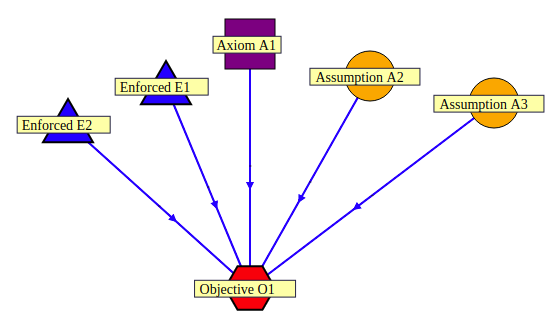
\includegraphics[width=8cm]{chainsaw.png}
\caption{Dependency graph of chainsaw assumptions, axioms, enforced conditions, and objective}
\label{chainsawdependence}.
\end{figure}

It is not necessary to make this proof any more clear. 

However, if we want to understand how the reasoning in this proof can
be represented in the predicate calculus, we must make it clear what
are the predicates, and re-express the axioms, assumptions, enforced
conditions, and objectives, using these predicates.  The predicates are
defined in Table \ref{chainsawpredicates} and the axioms etc, can then
be expressed as follows. Some subtle changes (including an additional
axiom) have emerged in the course of this translation.

iffalse
\begin{table}
\centering
\caption{Predicates used to ensure safety of chainsaw operation}\label{chainsawpredicates}
\begin{tabular}{|@{\tt}l|@{\hspace{5mm}}p{7cm}|}
\hline
\bf Predicate&\bf Meaning\\
\hline
Contact(x,y)& $x$ is a chainsaw which contacts human $y$\\
Braked(x)& The brake of chainsaw $x$ is on\\
UseOnTimber(x,y)& The chainsaw $x$ is in use by human $y$\\
Trained(x)& The operator $x$ has been trained\\
RearUp(x)& The chain saw $x$ rears up\\
ChainRunning(x) & The chain of chain saw $x$ is running\\
ChainRunning(x,h) & The chain of chain saw $x$ is running, under operator $h$\\
\hline
\end{tabular}
\end{table}

{\bf Axioms}
\begin{enumerate}[{A}1.]
\item\label{A1a} $\forall c, h, \left(\hbox{\tt Contact(c,h)} \wedge 
		\hbox{ChainRunning(}c{\tt )}\right) 
\supset\big( (\neg {\tt braked(c)} \wedge$\\
$ \neg\exists h_2,{\tt UseOnTimber(c,h_2)}) \vee (\exists h_3,{\tt UseOnTimber(c,h_3)}$\\ 
	$\wedge {\tt RearUp(c)})\big)$.
\item\label{A1b} $\forall c, {\tt braked(c)} \supset (\neg\exists h,{\tt ChainRunning(c,h)})$.
\item\label{A1c} $\forall c, h, {\tt ChainRunning(c,h)} \supset \neg\exists h_1\not=h, {\tt ChainRunning(}c,h_1
		{\tt )}$.
% \item\label{A1b} $\forall c: {\tt braked(c)} \supset (\neg{\tt UseOnTimber(c)})$.
% \end{enumerate}

\hspace{-9mm}{\bf Assumptions}

% \begin{itemize}
\item\label{A2a} $\forall h,c: {\tt Trained(h)} \supset \neg\exists c:\left(\neg {\tt UseOnTimber(c,h)} \wedge \neg{\tt braked(c)} \right)$
\item\label{A3} $\forall c: {\tt RearUp(c)} \supset {\tt braked}(c)$.
\end{enumerate}

{\bf Enforced conditions}

\begin{enumerate}[{E}1.]
\item\label{E1} 
$\forall h,c: {\tt Trained}(h) \supset \left( {\tt UseOnTimber(c,h)} \vee {\tt braked(c)} \right)$.

\item\label{E2} $\forall h, c: (\neg{\tt Trained(h)}) \supset (\neg{\tt ChainRunning(c,h)})$.

\item\label{E3} ${\tt ChainRunning(}c{\tt )} \supset \exists h,{\tt ChainRunning}(c,h{\tt )}$.
\end{enumerate}

{\bf Objective}

\begin{enumerate}[{O}1.]
\item\label{O1} $\forall c,h: \neg\left({\tt Contact(c,h)} 
		\wedge \big({\tt ChainRunning(}c{\tt )}\big)\right)$.
\end{enumerate}

In preparation for proving O\ref{O1}, we first prove:

\begin{proposition}\label{chrun--trained}
		${\tt ChainRunning}(c,h) \supset {\tt Trained}(h)$.
\end{proposition}

\begin{proof}
		This is the contrapositive of E\ref{E2}.
\end{proof}

\begin{proof}
Now that we have predicates to express the axioms, assumptions, etc, we can express the proof 
more rigorously. The proof is essentially the same (although some subtle mistakes will now
be corrected). 

Let's use proof by contradiction, i.e. we assume 
\begin{equation}\label{assumedforcontradiction}
{\tt Contact(}c_0,h_0{\tt )} 
\wedge {\tt ChainRunning(}c_0{\tt )}
\end{equation}
for some $h_0$ and $c_0$, 
and then show that this leads to a contradiction.

By A\ref{A1a}, it follows that either 
\begin{eqnarray}\label{conjunction} \nonumber
&&\neg{\tt braked}(c_0) \wedge \neg \exists h_2,{\tt UseOnTimber(}c_0,h_2{\tt )}\\
\noalign{~~~~~~~~~~or~}
		&&\left(\exists h,{\tt UseOnTimber(}c_0, h{\tt )}\right) \wedge {\tt RearUp(}c_0{)}
\end{eqnarray}

Let us consider the first of these two cases, 
\begin{equation}\label{notbrakedorinuse}
		\neg{\tt braked}(c_0) \wedge \neg\exists h_2,{\tt UseOnTimber(}c_0,h_2{\tt )}.
\end{equation}
In plain English, ``The chain is not braked, and the chainsaw is not being used to cut wood.''
By the second part of (\ref{assumedforcontradiction}) and E\ref{E3},
\begin{equation}\label{someonemustberunningit}
	\exists h_1, {\tt ChainRunning(}c_0,h_1{\tt )}.
\end{equation}
(E\ref{E3} is due to the fact that unless someone is pressing
the trigger of a chainsaw, the chain will not run. This is a second safety feature of chainsaws.)
By Proposition \ref{chrun--trained}, we conclude that for some $h_1$,
${\tt Trained(}h_1{\tt )}\wedge {\tt ChainRunning(}c_0,h_1{\tt )}$.
Hence, by A\ref{A1c}, 
$$
\neg \left( \exists h_1,\left({\tt ChainRunning(}c,h_1{\tt )}
\wedge \left(\neg{\tt Trained(}h_1{\tt )}\right) \right)\right).
$$
By E\ref{E1}, ${\tt ChainRunning}(c,h) \supset {\tt Trained}(h)$, and combining this
with A\ref{A1c}, we find 
\begin{equation}\label{mustbetrained}
{\tt ChainRunning}(c,h) \supset \forall h_1, \left( {\tt ChainRunning}(c,h_1) \supset {\tt Trained}(h_1)\right).
\end{equation}
Let $h_1$ be a human whose existence is asserted in (\ref{someonemustberunningit}). By (\ref{mustbetrained}), 
${\tt Trained}(h_1)$, so by E\ref{E1}, 
$$
\forall c: {\tt Trained}(h_1) \supset \left( {\tt UseOnTimber(c,h_1)} \vee {\tt braked(c)} \right),
$$
which contradicts (\ref{notbrakedorinuse}).

Now let us consider the second case, ${\tt UseOnTimber(}c_0{\tt )} \wedge {\tt RearUp(}c_0{)}$.
By (\ref{a&b->b}), ${\tt RearUp(}c_0{)}$. Hence, by A\ref{A3}, {\tt braked($c_0$)}. 
It therefore follows from A\ref{A2a}, that $\neg\exists h_0, {\tt ChainRunning(}c_0,h_0{\tt )}$.
But this contradicts our original assumption, ${\tt Contact(}c_0,h_0{\tt )} 
\wedge \exists h_0, {\tt ChainRunning(}c,h_0{\tt )}$. 
Thus, in both cases from the conjunction, (\ref{conjunction}),
we get a contradiction. Thus, the contradiction is confirmed, and we must conclude
that ${\tt Contact(}c_0,h_0{\tt )} \wedge \big(\exists h,{\tt ChainRunning(}c,h{\tt )}\big)$ is false.
\end{proof}

\end{sbexample}


\begin{exercise}{A theorem about the weather}%
Suppose ``John always carries an umbrella when rain has been forecast for the today''. Create 
logical predicates, which refer to a domain which includes John, and umbrellas,
and express this statement using formal logic.
Next, formulate and express, in formal logic, the statement: ``If John
is not carrying his umbrella, then rain was not forecast for today''.
Using logic, prove that this second statement follows from the first one.
\end{exercise}

\begin{exercise}{Logical Fallacies}
Identify which of the following arguments contain logical errors 
and, when there is an error, explain the mistake.
	\begin{enumerate}[(a)]
		\item % Mixing up contrapositives
John always carries his umbrella with him when rain is forecast, hence,
if we see John carrying his umbrella, rain must have been forecast.
		\item % Correct contrapositive
John always carries his umbrella with him when rain is forecast, hence,
if John is not carrying his umbrella, rain must not have been forecast.
		\item % Use of one example to prove a universal
Rain was forecast today and I see that Joan is carrying her umbrella, so,
Joan must always carry an umbrella when rain has been forecast.
		\item % Mis-calculated nots
On every day except Tuesday, Jim doesn't ride to work,
and he only has morning coffee before 10.00 am when he did not ride, 
hence on Tuesdays, if he has coffee, it will be after 10.00 am.
		\item % Use of one example to prove a universal (second case)
Our network was just broken into by an attacker who was an unhappy ex-employee
who was able to obtain administrator credentials through some inside information
about the IT operational procedures we used to practice. It follows that
this must be the main risk we need to protect against in future.
	\end{enumerate}
\end{exercise}


\begin{sbexample}{Device drivers and kernel modules}\label{kernelmodulesexample}%
All major operating systems (Linux, Microsoft Windows, MacOS, FreeBSD, and Android)
nowadays include {\em loadable kernel modules} \cite{loadableKernelModules}, 
which are extensions to the operating system
which can be added to, or installed, often without restarting the operating system.
Traditionally, this software runs with the same privilege level as the kernel itself.

Loadable kernel modules are extremely useful for enabling operating systems to adapt
to innovation in hardware, for example. A manufacturer of a device which provides a new
feature, for a phone, computer, or tablet, for example, can write and distribute a 
loadable kernel module which communicates with the device and enables software to use
it.

As a consequence, users are accustomed to installing new loadable kernel modules. Unfortunately,
if a loadable kernel module has a bug, or if it contains a security flaw (which might
be {\em deliberate}). Thus, the really useful feature of loadable kernel modules is
also. potentially, a serious flaw from the point of view of security.
\end{sbexample}

\begin{exercise}{Loadable kernel modules}\label{loadableKernelModulesExz}%
Think about what can be done to make loadable kernel modules safer. Make notes
recording your ideas. Then, try to find what has been done, in the industry, to address
this issue. Use the Wikipedia entry \cite{loadableKernelModules} on loadable kernel 
modules, in particular, as a starting point for your inquiries.
\end{exercise}

\begin{sbexample}{A formal system with predicates}\label{predicatesex}%
Now that we have introduced {\em predicates}, we can treat Example \ref{certificatesex}
more thoroughly, and develop a logical system which captures the logic of digital 
signatures both accurately and completely. The domain of objects here will include
{\em documents}, {\em signers}, {\em signatures}, {\em certificates}, and {\em certificate authorities}.
Note that the predicate calculus does not allow for the concept of differentiating
different {\em types} of object. 

Predicate calculus with types is possible, but would not introduced
significant changes from the point of view of logic. For more discussion of logic with
types, see Subsection \ref{logic_alternatives}\index{logic!typed}.

The predicates we need in this example are listed in Table \ref{certificatepredicates},
and the specific objects, and their names, used in the proof that Joan is a signatory,
are listed in Table \ref{joanobjects}.

\begin{table}
\centering
\begin{tabular}{|@{\tt}l@{\hspace{2mm}}|p{75mm}|}
\hline
\bf Predicate&\bf Meaning\\
\hline
HasSig(x,y)& $x$ is a document and $y$ is its signature\\
IsSignedBy(x,y,z)& $x$ is a document which is correctly signed by entity $y$ using certificate $z$\\
IsValidAccTo(x,y,z)& $x$ is a signature for document $y$ which is valid according to certificate $z$\\ 
IsValidSignatory(d,A,c)& $A$ is the signatory of the document $d$ according to 
the {\em valid} certificate $c$\\
IsValidSignatory(d,A)& $A$ is the signatory of the document $d$\\
HasCert(B,c)& $c$ is a certificate owned by $B$\\
IsValidCert(x)& $x$ is a valid certificate\\
IsValidAuth(X,x)& $X$ is a valid certificate authority according to their certificate, $x$\\
\hline
\end{tabular}
\caption{Predicates used to validate signatures}\label{certificatepredicates}
\end{table}


\begin{table}
\centering
\begin{tabular}{|@{\tt}l@{\hspace{2mm}}|p{6cm}|}
\hline
\bf Name&\bf Description\\
\hline
CA& Certisign digital certificate authority\\
VA& Verisign\\
cc& The certificate owned by Certisign which authorizes them as a certificate signing authority\\
js& Joan's certificate\\
ds& The signature on Joan's document\\
\hline
\end{tabular}
\caption{Names of objects and entities which appear in the proof that Joan is the signatory of the document}\label{joanobjects}
\end{table}

The axioms we identified in Example \ref{certificatesex} can now be written, more precisely:
\begin{enumerate}[{A}1]\small
		\item \label{A1}$\forall A, c, s, \exists ac:\hbox{\tt HasSig}(c,s) \wedge \hbox{\tt IsValidAccTo}(s,c,ac) \\
			\wedge \hbox{\tt IsValidSignatory}(c,A,ac) \supset \hbox{\tt IsValidCert}(c)$.
	\item \label{A2}$\forall A, d$, ac:\\
	$\left(\exists ds: \hbox{\tt HasSig}(d,ds) \wedge \hbox{\tt IsValidAccTo}(ds,d,ac) \wedge \hbox{\tt HasCert}(A,ac)\right) \\
			\supset \hbox{\tt IsSignedBy}(d,A,ac)$.
	\item \label{A3}$\forall A, d,ac: \hbox{\tt IsSignedBy}(d,A,ac) \wedge \hbox{\tt IsValidAuth}(A,ac) \\
			\supset \hbox{\tt IsValidSignatory}(d,A,ac)$.
	\item \label{A4}
$\forall A, c: \hbox{\tt HasCert}(A,c) \wedge \hbox{\tt IsValidCert}(c) \supset \hbox{\tt IsValidAuth}(A,c)$.
	\item \label{A5}
			$\left(\exists c: \hbox{\tt IsValidSignatory}(\hbox{\tt d},\hbox{\tt A},\hbox{\tt c})\right) \equiv
\hbox{\tt IsValidSignatory}(\hbox{\tt d},\hbox{\tt A})$.
	\item \label{A6}
			$\forall c, \hbox{\tt HasCert}(VA,c) \supset \hbox{\tt IsValidAuth}(\hbox{\tt VA,c})$.
\end{enumerate}


The enforced conditions, using the predicates listed in Table 
\ref{certificatepredicates}, can be stated as follows:
\begin{eqnarray}\nonumber
\textup{$E_1$}:&&\hspace{-5mm}\parbox{10cm}{{\tt HasSig(d,ds)}}\\ \nonumber
\textup{$E_2$}:&&\hspace{-5mm}\parbox{10cm}{{\tt IsValidAccTo(ds,d,jc)}}\\\nonumber
\textup{$E_3$}:&&\hspace{-5mm}\parbox{10cm}{{\tt HasCert(J,jc)}.}\\\nonumber
\textup{$E_4$}:&&\hspace{-5mm}\parbox{10cm}{{\tt HasSig(jc,jcs)}}\\ \nonumber
\textup{$E_5$}:&&\hspace{-5mm}\parbox{10cm}{{\tt IsValidAccTo(jcs,jc,cc)}}\\ \nonumber
\textup{$E_6$}:&&\hspace{-5mm}\parbox{10cm}{{\tt HasCert(CA,cc)}}\\ \nonumber
\textup{$E_7$}:&&\hspace{-5mm}\parbox{10cm}{{\tt HasSig(cc,ccs)}}\\ \nonumber
\textup{$E_8$}:&&\hspace{-5mm}\parbox{10cm}{{\tt IsValidAccTo(ccs,cc,vc)}}\\ \nonumber
\textup{$E_9$}:&&\hspace{-5mm}\parbox{10cm}{{\tt HasCert(VA,vc)}}\\ \nonumber
\end{eqnarray}


To break the proof of O into small peices, we introduce the following
intermediate propositions:

\begin{eqnarray}\nonumber
\textup{$p_1$}:&&\hspace{-5mm}\parbox{10cm}{{\tt IsValidAuth(VA,vc)},}\\ \nonumber
\textup{$p_2$}:&&\hspace{-5mm}\parbox{10cm}{{\tt IsValidSignatory(cc,VA)},}\\ \nonumber
\textup{$p_3$}:&&\hspace{-5mm}\parbox{10cm}{\tt IsValidAuth(CA,cc),}\\\nonumber
\textup{$p_4$}:&&\hspace{-5mm}\parbox{10cm}{{\tt IsValidSignatory(jc,CA)},}\\ \nonumber
\textup{$p_5$}:&&\hspace{-5mm}\parbox{10cm}{\tt IsValidAuth(J,jc).}\\\nonumber
\end{eqnarray}


{\bf Proof}
\begin{enumerate}[1.]
		\item{}\label{step1}
$p_1$: {\tt IsValidAuth(}VA,vc{\tt )}

By $E_9$, {\tt HasCert(}VA,vc{\tt )}, so by A\ref{A6},
{\tt IsValidAuth(}VA,vc{\tt )}. 

\item{}\label{step2} 
%\iffalse
$p_2$: {\tt IsValidSignatory(}cc,VA{\tt )}\\[5mm]

Using (\ref{specialization}), we can infer a version of A2 with {\tt cc} substituted for $d$,
{\tt VA} substituted for $A$, and {\tt ccs} substituted for $s$:
\begin{eqnarray}\label{A1a}\nonumber
&&\hspace{-7mm}\hbox{\tt HasSig(cc,ccs) $\wedge$ IsValidAccTo(ccs,cc,vc)$\wedge$ HasCert(VA,vc)} \\
		&&\hspace{-7mm}\nonumber
\supset \hbox{\tt IsSignedBy}({\tt cc, VA, vc}).
\end{eqnarray}

Now the first of the LHS terms is $E_7$, the second is $E_8$, and the third is $E_{9}$.
So by m.p., {\tt IsSignedBy}({\tt cc, VA, vc}). Now, using A\ref{A3}, and $p_1$, we conclude
that \hbox{\tt IsValidSignatory}({\tt cc, VA}).
%\else
%See Exercise \ref{step2ex}.
%\fi


\item{}\label{step3} 
$p_3$: {\tt IsValidAuth(}CA,cc{\tt )}
\iffalse

By $E_7$: {{\tt HasSig(cc,ccs)}};
$E_8$: {{\tt IsValidAccTo(ccs,cc,vc)}};
and $p_2$: {\tt IsValidSignatory(}cc,VA,vc{\tt )};
and A\ref{A1}, {\tt IsValidCert(}CA,cc{\tt )}. 

By $E_6$, {\tt HasCert(}CA,cc{\tt )}, so by A\ref{A4},
{\tt IsValidAuth(}CA,cc{\tt )}. 
\else
See Exercise \ref{step3ex}.
\fi

\item{}\label{step4} 
$p_4$: {\tt IsValidSignatory(}jc, CA{\tt )}
\iffalse

Using (\ref{specialization}), we can infer a version of A2 with {\tt jc} substituted for $d$,
{\tt CA} substituted for $A$, and {\tt jcs} substituted for $s$:
\begin{eqnarray}\label{A1a}\nonumber
&&\hspace{-7mm}\hbox{\tt HasSig(jc,jcs) $\wedge$ IsValidAccTo(jcs,jc,cc)$\wedge$ HasCert(CA,cc)} \\
		&&\hspace{-7mm}\nonumber
\supset \hbox{\tt IsSignedBy}({\tt jc, CA, cc}).
\end{eqnarray}

Now the first of the LHS terms is $E_4$, the second is $E_5$, and the third is $E_{6}$.
So by m.p., {\tt IsSignedBy}({\tt jc, CA, cc}). Now, using A\ref{A3}, and $p_3$, we conclude
that \hbox{\tt IsValidSignatory}({\tt jc, CA}).
\else
See Exercise \ref{step4ex}.
\fi
%

\item{}\label{step5} 
$p_5$: {\tt IsValidAuth(J,jc).}
\iffalse

By $E_4$: {{\tt HasSig(jc,jcs)}};

$E_5$: {{\tt IsValidAccTo(jcs,jc,cc)}};
$p_4$: {\tt IsValidSignatory(}cc,J,jc{\tt )};
and A\ref{A1}, {\tt IsValidCert(}J,jc{\tt )}. 

By $E_3$, {\tt HasCert(}J,jc{\tt )}, so by A\ref{A4},
{\tt IsValidAuth(}J,jc{\tt )}. 
\else
See Exercise \ref{step5ex}.
\fi


\item{}\label{step6} 
$O_1$: {\tt IsValidSignatory(d,J)}.

Using (\ref{specialization}), we can infer a version of A2 with {\tt d} substituted for $d$,
{\tt J} substituted for $A$, and {\tt ds} substituted for $s$:
\begin{eqnarray}\label{A1a}\nonumber
&&\hspace{-7mm}\hbox{\tt HasSig(d,ds) $\wedge$ IsValidAccTo(ds,d,jc)$\wedge$ HasCert(J,jc)} \\
		&&\hspace{-7mm}\nonumber
\supset \hbox{\tt IsSignedBy}({\tt d, J, jc}).
\end{eqnarray}
As before, the LHS elements of this inference have already been proved in $E_1$, $E_2$, and $E_3$,
so \hbox{\tt IsSignedBy}({\tt d,J,jc}) is true. Now, using A\ref{A3}, and noting that
have already shown $p_5$: {\tt IsValidAuth(J,jc).}

This proves $O_1$.
%
%
\end{enumerate}

The inference graph which connects each proposition, condition, axiom, or objective to the 
propositions, conditions, etc, that follow from them, in this example, is shown in Figure
\ref{certificateinfgraph}.

\begin{figure}
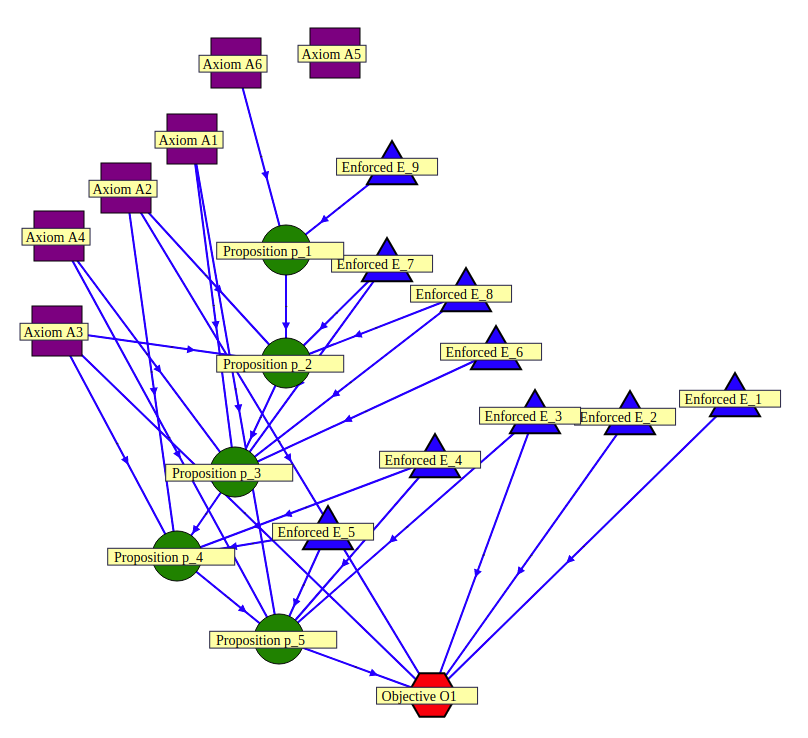
\includegraphics[width=12cm]{certificate2}
		\caption{The proof-dependency graph for the proof of objective $O_1$ from the enforced conditions
		and axioms, for Example \ref{predicatesex}}\label{certificateinfgraph}
\end{figure}
\end{sbexample}

\begin{exercise}{A Proof I}\label{step3ex}
Prove Item \ref{step3} from Example \ref{predicatesex}.
\end{exercise}
\iffalse
\begin{answer}{}
$p_3$: {\tt IsValidAuth(}CA,cc{\tt )}

By $E_7$: {{\tt HasSig(cc,ccs)}};
$E_8$: {{\tt IsValidAccTo(ccs,cc,vc)}};
and $p_2$: {\tt IsValidSignatory(}cc,VA,vc{\tt )};
and A\ref{A1}, {\tt IsValidCert(}CA,cc{\tt )}. 

By $E_6$, {\tt HasCert(}CA,cc{\tt )}, so by A\ref{A4},
{\tt IsValidAuth(}CA,cc{\tt )}. 
\end{answer}
\fi

\begin{exercise}{A Proof II}\label{step4ex}
Prove Item \ref{step4} from Example \ref{predicatesex}.
\end{exercise}
\iffalse
\begin{answer}{}
$p_4$: {\tt IsValidSignatory(}jc, CA{\tt )}

Using (\ref{specialization}), we can infer a version of A2 with {\tt jc} substituted for $d$,
{\tt CA} substituted for $A$, and {\tt jcs} substituted for $s$:
\begin{eqnarray}\label{A1a}\nonumber
&&\hspace{-7mm}\hbox{\tt HasSig(jc,jcs) $\wedge$ IsValidAccTo(jcs,jc,cc)$\wedge$ HasCert(CA,cc)} \\
		&&\hspace{-7mm}\nonumber
\supset \hbox{\tt IsSignedBy}({\tt jc, CA, cc}).
\end{answer}
\fi

\begin{exercise}{A Proof III}\label{step5ex}
Prove Item \ref{step5} from Example \ref{predicatesex}.
\end{exercise}

\iffalse
\begin{answer}{}
$p_5$: {\tt IsValidAuth(J,jc).}

By $E_4$: {{\tt HasSig(jc,jcs)}};

$E_5$: {{\tt IsValidAccTo(jcs,jc,cc)}};
$p_4$: {\tt IsValidSignatory(}cc,J,jc{\tt )};
and A\ref{A1}, {\tt IsValidCert(}J,jc{\tt )}. 

By $E_3$, {\tt HasCert(}J,jc{\tt )}, so by A\ref{A4},
{\tt IsValidAuth(}J,jc{\tt )}. 
\end{answer}
\fi



\subsection{The Syntax of Formal Logic}

The syntax of the propositional and predicate calculus is not dissimilar to that of a modern
progamming language. Close attention was paid to its syntax, because from the {\em formalist}
point of view, absolute clarity in these details was essential. 


According to the {\em formalist} interpretation of mathematics, mathematics
is {\em conceptually} nothing more than the manipulation of symbols according to the rules of
the predicate calculus. This is a highly artificial interpretation of mathematics and does
not genuinely represent mathematical thought. This idea was primarily entertained as a way
to justify reasoning concerned with infinite quantities (like the set of all natural numbers,
or the set of all real numbers), without having to justify the existence of these abstract
concepts.

For this reason, great care has been taken to define the syntax of the
predicate calculus.  Since neither computers, nor computer languages,
existed when the predicate calculus was developed, methods for describing
its syntax had to be developed.  We refer the reader to texts on logic,
like \cite{Kleene52}, \cite{Mendelson64} for these details.  It should
be noted that we have introduced one small variation from conventional
practice, which is that we use multi-character names for predicates, and
objects. This has been done to make their interpretation easier. Brevity
should not take precedence over clarity in the present context.

%Hand book-ch2 end
\subsection{cybersecurity architecture}
The concept that cybersecurity architecture is the discovery, definition and validation of {\em rules} (mandatory objectives and their conditions) is introduced.

\subsection{Inference graphs}\label{inferencesec}
The new concept of {\em inference graphs} for illustrating the relationship between cybersecurity rules is defined. The collection of cybersecurity rules forms a graph, in which the vertices represent cybersecurity rules, and the edges represent {\em inference}, in the sense that the collection of vertices with edges {\em terminating} at a certain vertex, $V$ for example, correspond to the set of rules which are sufficient to prove the rule corresponding to $V$. This representation of cybersecurity provides a way to develop cybersecurity architecture\cite{Rerup2018}. These diagrams can also be used in security design, as a way to validate security designs, for documentation, and as a way to visualise and develop alternative designs.

An inference graph shows the relationship of {\em inference} (what implies what) which applies to the different cybersecurity rules which apply in a system.
Examples of inference graphs are shown in Figures \ref{parcelboxrules}  and \ref{certificaterulesgraph}. These will be explained in Section \ref{examplesec}.

The following types of rules arise in cybersecurity analysis: {\em objective}, {\em enforced rule}, {\em axiom}, {\em proposition}, and {\em assumption}. An objective is a rule which is required to be true at all times. An enforced rule is a condition that is possible to enforce, and which it has been decided to enforce, by technical means. For example, access to many systems is only provided if a user is able to enter a valid username and password.

An axiom is a condition that is held to be true {\em a priori}; an assumption is a condition which we {\em choose} to believe. For example, under some conditions, we assume that users do not reveal their password to other users. A proposition is a rule or statement which we define in order to express a useful stage of reasoning.

An {\em edge} in an inference graph connects each of the rules referenced in proof to the rule which is proved. Objectives are typically the destination of edges, while enforced rules usually occur only as of the origin of an edge.

\subsubsection{Proof as a relationship}
The {\em goal} of cybersecurity is to guarantee that certain objectives are maintained. For example, it is likely that a bank will have, as an objective, that no transactions -- transfers of money from one account to another -- occur except with valid authorization.

The aim of cybersecurity {\em design} is to discover or instantiate axioms, assumptions, and enforced rules which enable us to {\em prove} that the {\em objectives} are true. Along the way to doing this, there may be some {\em intermediate propositions} that we also wish to prove.

Thus, {\em objectives} and {\em intermediate propositions} have proofs. On the other hand, {\em axioms} do not have proofs because these are fundamental truths that are true from logical principles or, in some cases, because they express follow from the definition of the predicates they contain, {\em assumptions} are true by assumption (which might not always hold, but at present we adopt them), and {\em enforced rules} are true because we make sure, in the system, that they are true, so none of these rule types has proofs.

The appearance of a reference to a proposition, assumption, axiom, objective, or enforced rule, in a proof,  constitutes a relationship between that rule and the rule is proved. The {\em inference graph} has vertices or nodes corresponding to the rules and directed edges or links from any rule which is referenced in proof to the rule which is proved.


In the diagrams which are included below, the different types of rules are represented by nodes of different shapes and colours, as  indicated in the Legend, shown in Fig. \ref{legend}. \begin{figure}[bhpt]
	\centering
		\leavevmode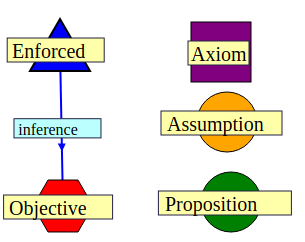
\includegraphics[width=42mm]{legend.png}\ \\
		\caption{Legend for Inference graphs}\label{legend}
\end{figure}




\subsection{Examples of inference graphs}
Three increasingly complex examples of inference graphs for systems needing cybersecurity architecture are presented, including the detailed proofs which form the basis of these inference graphs, in some cases. 

We see how a key design objective is achieved rigorously by a clever decision that emerges from the use of the cybersecurity inference graph of this system. Example 2 is based on a cybersecurity weakness in a web service administered by one of the authors, which was analysed and solved previously \cite{exptsandproofs} so in this case, the inference graph is used to illustrate the proofs which were developed then. In Example 3, finding the correct proofs was a complicated task which was facilitated by the use of the inference graph of rules and objectives of the system.}



\subsection{Inference Graphs Software}
 
The software which has been developed to support the development and use of cybersecurity inference graphs is described including details of the public server where it can be used. 

\subsection{Conclusion}
In this section and Chapter 5, we tried to show that cybersecurity inference graphs can significantly contribute to the development of, and validation of cybersecurity and also that rigorous validation of cybersecurity is not necessarily as complex as previously thought.

\section{Experiments using examples}
\iflonger
\subsection{security audit}
An approach used periodically is to assign the task of attack or harm   a service in cyber space  to an individual or a team and then address the discovered weaknesses. We call this a {\em security audit}. The approach of searching for weaknesses and fixing them is so widely used that it might reasonably be regarded as a design philosophy.
This approach has been used in this dissertation, and the results of
both the attacks and the resulting defences are reported.
However, this approach is somewhat pessimistic in that it {\em assumes}
that a more methodical security design philosophy which can guarantee
secure design is not available.
\fi

\section{Gathering ideas and reviewing ideas from literature}


An important methodology in this dissertation, as in all scientific work, is to gather the thoughts of other researchers, who are struggling with the same problems as tackled here, and to identify key ideas and principles that have previously been suggested, and to recognise the most important of these and make use of them in this work.
\if
Because web services (including services provided via apps on mobile phones)
are a recent development and continue to evolve in both details and fundamentals,
principles of secure design of these services is also a new and evolving area of
research and development \cite{AddieColman2010,Addie_Moffatt_Dekeyser_Colman2011}.
\else\cite{Addie_Moffatt_Dekeyser_Colman2011}.
\fi

This section reviews three different approaches for securing web sites/services.
Each of these approaches is usually expressed as a completely independent
philosophy for achieving good security. We shall see that these approaches 
are actually complementary, and to achieve rigorous security all three approaches
are needed. Note that although we describe a design philosophy which is able, formally, to prove,
i.e.  guarantee, security, because no logical system can claim certainty in an absolute
sense (in mathematical logic, this fact is expressed in G\"odel's incompleteness theorem), the strategy 
of attacking the system remains useful, even after it has been
methodically proved to be correct.

The present paper does not apportion equal emphasis on all approaches
because the original contribution of this paper is 
in the third of them, together with the way the second approach joins
with the third to form a more comprehensive whole. The second approach
is the one summarised in Subsection \ref{audit} and applied
in Section \ref{expts}.
The third approach is summarised in Subsection \ref{stsecanal} and applied
to the Netml password reset system in Sections \ref{stakeholders} and \ref{proof}.

%\subsection{Web Service Security Design}\label{webservicessecurity}







\subsection{Good Security Design Practice}
Good design takes security, ease of access, and usability into account,
striking a balance between protecting the system and ease of use. Good
practice has evolved a number of practical approaches like  minimizing
attack surface area \cite{bhardwaj2018reducing},  establish secure
defaults \cite{lai2018impact}, using the principle of defence in depth
\cite{toch2018privacy}, not trusting services \cite{ghirardello2018cyber},
keeping security simple \cite{thomsen2018network}, and fixing security
issues correctly \iflonger\cite {ali2018security, tabassum2018evaluating}.
\else \cite {tabassum2018evaluating}.\fi
These approaches  are used for  maintaining and improving security which
are so natural and important that they should be adopted as a first
layer of protection as a matter of standard practice, even when more
sophisticated approaches are also in use \cite {ross2018systems}.


\subsection{Security Auditing}\label{audit}

Strategies for breaking into web systems or services are under continuous
development by government and non-government organisations and individuals,
both those with friendly intentions and those who wish to exploit security
weaknesses for their own advantage. When
a new exploit is discovered, if it is discovered first by those with 
friendly intentions, defences against the exploit are usually developed
quickly and published. Exploits discovered by attackers with ill intent
can, of course, be deployed before web managers have the opportunity
to defend against them. Also, in the period of time immediately after
the defence against a new exploit has been published, there is still
an opportunity to attack web sites which have not deployed the newly developed
defences. This time can be somewhat extended due to the limitated expertise
of web-site owners and because the sequence of steps required to address a weakness
in a high-level framework can be quite lengthy.

A widely used strategy for improving web site or web service security is
to attempt to attack the site by using the strategies which are currently
known to be effective one-by-one, or simultaneously, to discover if the
site is vulnerable to any of these strategies. Since all of the strategies
tried are known, the defences against all of them are also almost certainly
known, and hence can be adopted by the web site.

Experiments of this type, and the resulting web service design improvements,
are described in Section \ref{expts}.



\subsection{Stakeholder Security Analysis}\label{stsecanal}

A more fundamental strategy which is not well-developed at present is
to seek to develop provably secure protocols and software for all aspects
of a web service \cite{whitman2011principles,mailloux2018examination,bishop2005introduction}.

The first step in this approach, which is developed further in 
Section \ref{stakeholders}, is to consider the point of view of all legitimate stakeholders
in relation to the service, and to enumerate a complete set of rules
required by each of these stakeholders, sufficient to ensure that they
will agree to actively participate in the service.


\section{Stakeholder Security Analysis}

[Stakeholder security analysis is a more specific form of logical analysis. Instead of dealing with
objectives in general, it makes use of the obvious but useful fact that all systems have
stakeholders, and the objectives of the system as a whole can be sub-divided into those
which can be ascribed to each stakeholder. Once their objectives have been identified, they
can be further analysed, refined, and reviewed. In particular, it is important to work out if
their objectives are compatible.]
The main result of this dissertation is to demonstrate  a secure methodical design philosophy.
We call this {\em stakeholder security analysis}.
\iffalse
%Hand book-----ch2-2.3.1 begin
Every business, organization, or community has {\em stakeholders}. These are the people (or agents) who have an interest in any aspect of its operation. In many cases, there will be a large group of {\em clients}, i.e. individuals who receive a service. There may be one or more {\em owners}. There are also many other ways a person, agent, or entity can have an interest in a given organisation or entity. One organization can be a stakeholder in another.
%Hand book-----ch2-2.3.1 end
\fi
In this section, we designed stakeholders' policies to incorporate human
values and ethics as much as possible into software values

Stakeholder security analysis proceeds as follows: 
\begin{enumerate}[1.]
\item Identify the key stakeholders.
\item For each stakeholder, identify a set of rules {\em required}
by these stakeholders. Note: the collected rules required
by all stakeholders must be consistent.
\item Implement procedures which ensure that all rules are enforced.
\end{enumerate}

Both a security audit and a stakeholder security analysis
are applied in this dissertation to a specific subsystem of a web
service system being developed and managed by the authors.
Note: it is not suggested that stakeholder security analysis obviates
the need for a security audit.



\subsubsection{Modular Security}\index{security!modular}

Because security tends to deal with absolutes, i.e. the rules to be assumed, or enforced, are true or false, it is tempting to imagine that the entire system must be either secure or not secure. This is an instance of the autocracy fallacy. According to this point of view, the only possible political system, for efficiency and correctness, is autocracy. Ideally, the person in charge should be {\em me}, because then no mistakes can happen.

However, in reality, almost all the computer and human systems with which we have to deal are imperfect. This includes their security. Real systems have security flaws, and yet they continue to function and provide service. When their flaws are discovered, we should endeavour to ensure that they are fixed as quickly as possible. But there is no need to pretend that such flaws do not exist. Furthermore, a security flaw in one aspect does not necessarily mean that security in any other area is also flawed.

The method of analysis and design of security outlined in this Chapter can be applied, methodically, to a {\em component} of the whole system, with a view to creating, implementing, and validating a design that achieves its intended security objectives.
\iffalse
\subsubsection{Stakeholder Business Rules}\label{stbsnrul}
Business rules refer to any rule relating to the way in which transactions are restricted. Business rules must be observed when designing and improving system security. In other words, even if the proposed security rules are enforced, they must be considered to be subject to the satisfactory standard by their professional organization. It is necessary to focus on Business rules  which are explicit rules on safety and try to study them and analyze them before drafting the security rules to avoid the contradiction.
The expectations of stakeholders which constitute a security case are considered mandatory and must be included in a security rule.
\fi
\subsubsection{Business Rules}\index{rule!business}

The analysis method investigated in this section makes use of {\em rules} which define the security of the system. The use of rules is not confined to security.
A {\em rule} is {\em defined} in this book to mean any statement which defines
a condition. In most cases, such rules are defined because it is intended that the condition {\em holds}, i.e. It is true, all the time. In some cases, this may be because it is {\em enforced}. In other cases, it is because it might follow other rules which are enforced. And of course, we shall consider cases where rules fail to hold, also.

An example of a business rule which is not necessarily a security rule is: {\em all customers must pay for their meals before collecting them}. 

The boundary between business rules which are concerned with security and those which are not may be unclear. When in doubt, the rule might need to be included with the security rules. This is because the purpose of security rules is to maintain the conditions for the mandatory objectives of the stakeholder, and if a {\em business rule} is required, for this well-being, then it must be maintained also.
\iffalse
\subsubsection{Business Rules}\index{rule!business}

The analysis method investigated in Chapter \ref{analysischap} makes use of {\em rules} which define the security of the system. The use of rules is not confined to security.
A {\em rule} is {\em defined} in this book to mean any statement which defines
a condition. In most cases, such rules are defined because it is intended that the condition {\em holds}, i.e. It is true, all the time. In some cases, this may be because it is {\em enforced}. In other cases, it is because it might follow other rules which are enforced. And of course, we shall consider cases where rules fail to hold, also.

An example of a business rule which is not necessarily a security rule is: {\em all customers must pay for their meals before collecting them}. 

The boundary between business rules which are concerned with security and those which are not may be unclear. When in doubt, the rule might need to be included with the security rules. This is because the purpose of security rules is to maintain the conditions for the mandatory objectives of the stakeholder, and if a {\em business rule} is required, for this well-being, then it must be maintained also.
\fi

\subsubsection{Service Protection Rules}\index{service!protection}\index{rule!service protection}

In the provision of services, which is a component of many businesses, it is frequently necessary to define and manage the performance with which the service is provided. For example: {\em Pizzas will be delivered within 15 minutes of leaving the oven.} As with other business rules, such rules cannot necessarily be separated neatly from security, or, if there is such a separation, it may lead to inappropriate strategies for achieving security objectives. For example, if the rules defining security are considered in isolation, without considering performance, simply denying access for {\em all} users might be considered a perfect security design.

Rules which define the level of service which should be achieved by a system or service are termed {\em service protection rules}.

\subsubsection{Objectives and Constraints}

In Operations Research, one of the most successful methodologies, over several decades, is {\em optimization}. In this framework, a problem is defined by two features: (i) an {\em objective}, and (ii) the {\em constraints}. These features define an optimization problem, the solution of which is to find the design which maximizes the objective without failing to meet the constraints.

This framework enables us to create a rigorous, scientific framework for many real-world problems quite readily. We just have to find the constraints, and the objective, and then solve the optimization problem.

When we attempt to put security into this framework, it becomes clear that although it works, accurately, it fails to achieve the right emphasis. In security, the emphasis must be almost exclusively on the constraints. The constraints, in a security problem, are the rules: including business rules, service protection rules, and all the security rules required by the stakeholders. The objective will, in most cases, be obvious, but not particularly relevant.

It is usually felt that there are limited opportunities for achieving cost savings by searching for, or devising, better security strategies. There may be more such opportunities in the future, and this possibility should not, therefore, be entirely neglected. However, for the most part, the challenge, in security design, is not {\em minimizing cost}, or {\em maximizing profit}, but rather {\em achieving certainty}, that all required security rules have been enforced.


\subsection{Stakeholders}

Every business, organization, or community has {\em stakeholders}. These are the people (or agents) who have
an interest in any aspect of its operation. In many cases there will be a large group of {\em clients}, i.e. 
individuals who receive a service. There may be one or more {\em owners}. There are also many other ways
in which a person, agent, or entity can have an interest in an a given organization or entity. One organization
can be a stakeholder in another.

\subsection{Stakeholder Roles}\label{strol}
The roles are defined first, then their stakeholders, and access levels and features are set in those roles. Security rules are defined based on stakeholders roles, and not stakeholders themselves, where we can state the rule in terms of anyone who is playing a certain role. Stakeholder experiences should be shared to identify vulnerabilities that may occur while dealing with the service or part of the system under study. Most organizations consider the reputable more than the performance of their systems. Therefore, they adopt robust security solutions. However, access levels for sources as well as sensitive data often require additional restrictions above standard security requirements. Hence,  additional restrictions are identified and chosen with extreme care, ensuring their independence, and providing sources and data to the real interest without any other party who can access the current security restrictions.
\subsection{Stakeholders Rules}

Any business, organisation, club or association has {\em stakeholders}. A stakeholder is a person, or 
entity, with some interest in activities of the organisation. Typically, there will be 4-5 key stakeholders.

\begin{sbexample}{Stakeholders of a University}%
Consider a university, for example. Key stakeholders are: (i) students, (ii) staff (which may be further
subdivided into academic, administration, management, and support staff), (iii) employers of graduates,
(iv) governments, and (v) parents of students.
\end{sbexample}

Many of the rules expected or mandated by stakeholders fall into fairly standard categories, like
{\em legal requirements}, {\em ethics}, etc, which are fairly similar across different stakeholders.
Most of these requirements are well-known, but nevertheless, these requirements do call for 
rules that need to be enforced by security design. Therefore it is useful for us to consider these
requirements explicitly. We consider these generic rules first.

\subsubsection{Specific Stakeholder Rules}

Stakeholders of an institution have certain reasonable expectations that are
probably understood by the other stakeholders, or which they communicate to them
either explicitly, or by their actions. Many of these expectations will lead
to rules that are explicitly or implicitly imposed on the operation of the institution.

\begin{sbexample}{Stakeholder Rules for a University}%
Continuing with the previous example, let us explore the rules that the stakeholders of a university
expect (or insist) should hold.

{\bf Students}

Students enrol and attend university to receive an education. They expect this education to qualify
them to gain work in their field of study. 

In addition, students have reasonable expectations regarding their ability to succeed or excel.
They expect to be able to make use of and learn by means of the learning resources provided to
them, to be able to achieve better results by spending more time and focussing more effectively
on their studies. They expect their efforts to be rewarded fairly, relative to other students.
In particular, they expect students with poor understanding, or who attempt to succeed without
really engaging in the learning process in an effective or legitimate way to be identified and
to achieve significantly worse outcomes.



{\bf Staff}

Staff expect to receive satisfactory remuneration for their work, to be adequately resourced,
including satisfactory computing, and communication resources. They also expect their managers
to provide adequate guidance concerning their resonsibilities, and training to enable them
to complete their responsibilities with a high level of professionalism.


Staff expect records concerning themselves to be treated with appropriate care, and in particular,
such records should not be shared with others except for purposes which are reasonable and 
with which they are in accord.

{\bf Employers}

Employers expect graduates from a university to be able to communicate, and collaborate with
other employees. They expect graduates to behave ethically (and in particular, honestly) in relation
to their work, employer, clients and colleagues. The also expect graduates to have knowledge
and understanding in the technical area in which they were studying.

{\bf Governments}

Governments expect students to receive an education which enables them to gain employment and
make a sound contribution to their employers. They expect university staff to act with respect and
probity toward each other, and toward students.

{\bf Parents}

Parents expect universities to treat their children with respect, to provide them with 
a good education, assessed fairly, and without subjecting them to harrassment or
abuse of any kind.

\end{sbexample}

Much of what stakeholders expect and demand cannot actually be encapusulated in a {\em rule}.
This doesn't mean that we should ignore such expectations. However, these expectations
are not usually considered relevant to {\em cyber-security}. In general, it is only
the expectations which are a matter of insistence, i.e. these are mandatory requirements,
which we consider to be an issue of security.


\iffalse
\subsubsection{Stakeholder SWOT}\label{stswot}
The SWOT analysis tools are used to evaluate the security aspects for the stakeholders in the system Fig(). The first step is to determine the security objectives required by each stakeholders role and business rules within the specific service,Password Reset Service. And then identify the internal factors (strengths, weaknesses) and external factors (opportunities, threats) that are favourable and unfavourable to achieve those objectives.

Strengths are an opportunity to support security objectives, while weaknesses are considered to be the vulnerabilities that may impede the achievement of these objectives. The statement of the risks of weaknesses and the great efforts to fix them and clarify the strengths in the implementation of the security rules that prevent such circumstances are sufficient justification for obtaining the approval of the owners of the decision. On the other hand, the lack of funds and inconsistencies with business rules in achieving security objectives are weaknesses. In terms of opportunities, they are any initiatives available to support security objectives such as sources, expenditures, technologies, and security policies.Threats are related to the importance of the system and the sensitive information it contains. They often exploited weaknesses.


%These objectives support the protection of password reset service.
\subsubsection{Stakeholder Security Rules}\label{stsecrul}
\subsubsection{Assumption}\label{assmp} 
After completing security rules, assumptions are developed that simplify the logic necessary to complete the design process. The degree of simplification is determined depending on the sensitivity of the security issue. Security rules are therefore classified as optional or mandatory. Unlike the optional category, which is assumed or obvious assumptions, mandatory class assumptions are security requirements that need to be adopted in the design or development of system security.
\subsection{Stakeholder Security Design}\label{stsecdsgn} 
The main goal in the design phase is to know which of the mandatory security rules must be guaranteed and how to do it. When a particular  rule is not guaranteed directly,  this rule should be checked  that it follows from our assumptions and the rules which are enforced. However , there are three categories of rules: (i)assumptions; (ii) enforced rules; (iii)rules that must be proven, and through careful examining of the latter, the process of checking security becomes more reliable and systematic.

In addition, unrealistic assumptions may cause security vulnerability. Also, very strict assumptions can undermine security. However, the combination of the two methods can lead to simple and effective security design and achieve a higher security level in certain situations of critical importance.
\subsubsection{Inforcable Stakeholder Security Rules}\label{Instsecrul}
\subsubsection{Validation of Stakeholder Security Rules}\label{vlstsecrul}

[It is not always possible to prove hypotheses, even when there are strong reasons for believing
them to be true. In science, and even in mathematics, some valid hypotheses can only be demonstrated
by examples. A very good example of this sort of hypothesis is Church's thesis, which is that
all concepts of computability are equivalent to Turing computability. A very large number of papers
were written, in the past, which showed that this or that type of computability was equivalent to
Turing computability. Eventually, journals put a stop to such publications. The concept that there is
really just one type of computable function had been established. But it was not a provable concept.
It was necessary to prove it by examples.

There are other advantages of examples. They are also an ideal way to demonstrate ideas in a 
natural and attractive fashion.

In this dissertation, many examples will be used to illustrate ideas which are in an obvious
sense quite similar in multiple superficially different cases. The striking similarity, in
different contexts, demonstrates that the concept is not an accident, but represents an important
principle.]




\iffalse
\section{A social contract for cyberspace}
We proposed a social contract for cyberspace that can manage Stakeholders'
policies and ensure their respect by their owners.
\fi

\fi